%%Adaptação do template para TCC do CEFET-MG dos professores Daniel Hasan Dalip e Glívia Angélica 

%% Baseado no arquivo: 
%% abtex2-modelo-trabalho-academico.tex, v-1.9.6 laurocesar
%% by abnTeX2 group at http://www.abntex.net.br/ 
%% Adaptado para um modelo dssse TCC (Graduação)

% ------------------------------------------------------------------------
% ------------------------------------------------------------------------
% abnTeX2: Modelo de Trabalho Academico (tese de doutorado, dissertacao de
% mestrado e trabalhos monograficos em geral) em conformidade com 
% ABNT NBR 14724:2011: Informacao e documentacao - Trabalhos academicos -
% Apresentacao
% ------------------------------------------------------------------------
% ------------------------------------------------------------------------

\documentclass[
	% -- opções da classe memoir --
	12pt,				% tamanho da fonte
	openright,			% capítulos começam em pág ímpar (insere página vazia caso preciso)
	twoside,			% para impressão em recto e verso. Oposto a oneside
	a4paper,			% tamanho do papel. 
	% -- opções da classe abntex2 --
	%chapter=TITLE,		% títulos de capítulos convertidos em letras maiúsculas
	%section=TITLE,		% títulos de seções convertidos em letras maiúsculas
	%subsection=TITLE,	% títulos de subseções convertidos em letras maiúsculas
	%subsubsection=TITLE,% títulos de subsubseções convertidos em letras maiúsculas
	% -- opções do pacote babel --
	english,			% idioma adicional para hifenização
	%french,				% idioma adicional para hifenização
	%spanish,			% idioma adicional para hifenização
	brazil				% o último idioma é o principal do documento
	]{abntex2}

% ---
% Pacotes básicos 
% ---
\usepackage{lmodern}			% Usa a fonte Latin Modern			
\usepackage[T1]{fontenc}		% Selecao de codigos de fonte.
\usepackage[utf8]{inputenc}		% Codificacao do documento (conversão automática dos acentos)
\usepackage{lastpage}			% Usado pela Ficha catalográfica
\usepackage{indentfirst}		% Indenta o primeiro parágrafo de cada seção.
\usepackage{color}				% Controle das cores
\usepackage{graphicx}			% Inclusão de gráficos
\usepackage{microtype} 			% para melhorias de justificação
% ---
		

% ---
% Pacotes de citações
% ---
\usepackage[brazilian,hyperpageref]{backref}	 % Paginas com as citações na bibl
\usepackage[alf]{abntex2cite}	% Citações padrão ABNT

% --- 
% CONFIGURAÇÕES DE PACOTES
% --- 

% ---
% Configurações do pacote backref
% Usado sem a opção hyperpageref de backref
\renewcommand{\backrefpagesname}{%Citado na(s) página(s):~
}
% Texto padrão antes do número das páginas
\renewcommand{\backref}{}
% Define os textos da citação
\renewcommand*{\backrefalt}[4]{
	%\ifcase #1 %
	%	Nenhuma citação no texto.%
	%\or
	%	Citado na página #2.%
	%\else
	%	Citado #1 vezes nas páginas #2.%
	%\fi
    }%
% ---

% ---
% Informações de dados para CAPA e FOLHA DE ROSTO
% ---
\titulo{Primeiro Trabalho de Algoritmo e Estrutura de Dados : Resolução do Problema da Mochila Por Estratégia Gulosa e Tentativa e Erro}
\autor{Victor Franco Rezende}
\local{Belo Horizonte}
\data{2018}


\instituicao{%
  Centro Federal de Educação Tecnológica de Minas Gerais -- CEFET-MG
  \par
  Departamento de Computação
  \par
  Curso de Engenharia da Computação
  }

% O preambulo deve conter o tipo do trabalho, o objetivo, 
% o nome da instituição e a área de concentração 
\preambulo{Trabalho Prático da Disciplina de Algoritmos e Estruturas de Dados I ministrada pela professora Natália Batista.}
% ---


% ---
% Configurações de aparência do PDF final

% alterando o aspecto da cor azul
\definecolor{blue}{RGB}{41,5,195}

% informações do PDF
\makeatletter
\hypersetup{
     	%pagebackref=true,
		pdftitle={\@title}, 
		pdfauthor={\@author},
    	pdfsubject={\imprimirpreambulo},
	    pdfcreator={LaTeX with abnTeX2},
		pdfkeywords={abnt}{latex}{abntex}{abntex2}{trabalho acadêmico}, 
		colorlinks=true,       		% false: boxed links; true: colored links
    	linkcolor=blue,          	% color of internal links
    	citecolor=blue,        		% color of links to bibliography
    	filecolor=magenta,      		% color of file links
		urlcolor=blue,
		bookmarksdepth=4
}
\makeatother
% --- 

% --- 
% Espaçamentos entre linhas e parágrafos 
% --- 

% O tamanho do parágrafo é dado por:
\setlength{\parindent}{1.3cm}

% Controle do espaçamento entre um parágrafo e outro:
\setlength{\parskip}{0.2cm}  % tente também \onelineskip

% ---
% compila o indice
% ---
\makeindex
% ---

% ----
% Início do documento
% ----
\begin{document}

% Seleciona o idioma do documento (conforme pacotes do babel)
%\selectlanguage{english}
%\selectlanguage{brazil}

% Retira espaço extra obsoleto entre as frases.
\frenchspacing 

% ----------------------------------------------------------
% ELEMENTOS PRÉ-TEXTUAIS
% ----------------------------------------------------------



%% Baseado no arquivo: 
%% abtex2-modelo-trabalho-academico.tex, v-1.9.6 laurocesar
%% by abnTeX2 group at http://www.abntex.net.br/ 
%% Adaptado para um modelo de TCC (Graduação)

% ---
% Capa
% ---
\imprimircapa
% ---

% ---
% Folha de rosto
% (o * indica que haverá a ficha bibliográfica)
% ---
\imprimirfolhaderosto*
% ---



% \vspace{\onelineskip}

% FERRIGNO, C. R. A. \textbf{Tratamento de neoplasias ósseas apendiculares com
% reimplantação de enxerto ósseo autólogo autoclavado associado ao plasma
% rico em plaquetas}: estudo crítico na cirurgia de preservação de membro em
% cães. 2011. 128 f. Tese (Livre-Docência) - Faculdade de Medicina Veterinária e
% Zootecnia, Universidade de São Paulo, São Paulo, 2011.

% \begin{table}[htb]
% \center
% \footnotesize
% \begin{tabular}{|p{1.4cm}|p{1cm}|p{3cm}|p{3cm}|}
%   \hline
%    \textbf{Folha} & \textbf{Linha}  & \textbf{Onde se lê}  & \textbf{Leia-se}  \\
%     \hline
%     1 & 10 & auto-conclavo & autoconclavo\\
%    \hline
% \end{tabular}
% \end{table}

% \end{errata}
% ---



% ---
% RESUMO
% ---

% resumo em português
\setlength{\absparsep}{18pt} % ajusta o espaçamento dos parágrafos do resumo
\begin{resumo}
Este trabalho busca resolver o "Problema da Mochila", utilizando dos metódos de "tentativa e erro" e "aloritmos guloso". Então será apresentado uma análise sobre os algortimos apresentados. O problema é um problema clássico para programação dinâmica e desenvolvimento de software.
Logo após, apresente os resultados obtidos, contribuições e conclusões obtidas.

 \textbf{Palavras-chave}: Algoritmos. Programação Dinâmica. Mochila.
\end{resumo}



% ---
% inserir o sumario
% ---
\pdfbookmark[0]{\contentsname}{toc}
\tableofcontents*
\cleardoublepage
% ---

% ----------------------------------------------------------
% ELEMENTOS TEXTUAIS
% ----------------------------------------------------------
\textual

% ----------------------------------------------------------
% Como o documento será grande, sugiro dividir em diversos arquivos, um para cada capítulo.
% ----------------------------------------------------------


\chapter[Introdução]{Introdução}
\label{cap:introducao}

O problema da mochila é um problema de optimização combinatória. A situação pode ser descrita como preencher uma mochila com o maior valor possível uma vez que ela somente suporta um determinado peso e cada objeto tem um valor e peso bem definido.

Para este trabalho usamos as estratégias de algoritmos guloso e tentativa e erro. A aproximação pelo algoritmo guloso consiste em primeiro ordenar o vetor de alguma forma, seja por peso ou por valor e então tomar decisões baseadas nas informações com base elas são adquiridas, sem voltar atrás. Ou seja, uma vez que um objeto foi colocado na mochila, ele não poderá ser retirado. A aproximação por tentativa e erro, ou backtracking pode ser definida como criar uma árvore de possibilidades e então percore-la até que se ache a "saida" ou alguma solução viável. 

Ambos os algoritmos não apresentam soluções ótimas, porém são estrategias válidas.


\chapter[Algoritmos]{Algoritmos}
\label{cap:formato}

Este capítulo apresenta os algoritmos utilizados nesse trabalho e faz uma análise a discussão sobre a viabilidade/aplicabilidade de cada um deles. 

A entrada de dados foi padronizada para : Os n itens da loja serão fornecidos em um arquivo texto que contêm na primeira linha W (capacidade da mochila), na segunda linha n (número de itens) e nas linhas seguintes os itens, cada
um em uma linha (contendo o peso seguido do valor). Os valores devem ser números inteiros.

Enquanto a saida seria: 

a) um arquivo texto contendo, nesta ordem:
\begin{itemize}
\item para cada item escolhido para a solução, o número do item, seu peso e seu valor (uma
linha por item)
\item uma linha contendo o somatório dos pesos dos itens escolhidos
\item  uma linha contendo o somatório dos valores dos itens. 
\end{itemize}
b) a impressão na tela do tempo total de execução do programa.

Devido a essa padronização, de entradas e saídas, parte dos programas se repete.
\section{Algoritmo Guloso}
\label{sec:preTextual}
 O algoritmo guloso é geralmente descrito como um algoritmo \textit{míope}, pois toma decições baseado nas melhores esolhas locais, isso é, nunca olha os resultados dessa escolhas futuramente. Muitas poucas vezes os algoritmos gulosos apresentam resoluções ótimas, porém apresentam resoluções perto das ótimas em uma quantidade razoável de vezes. 
 
\subsection{Análise do Algoritmo}
 A Figura 1 representa a esquematização do algoritmo, onde se aplica cria o TAD (tipo abstrato de dado) Objeto, que é composto de um peso e um valor. Após a criação de um vetor de Objetos, se organiza esse vetor e aplica o vetor ordenado na função Guloso, que retorna o resultado.

\begin{figure}[htb!]
    \centering
    \caption{Algoritmo Guloso}
    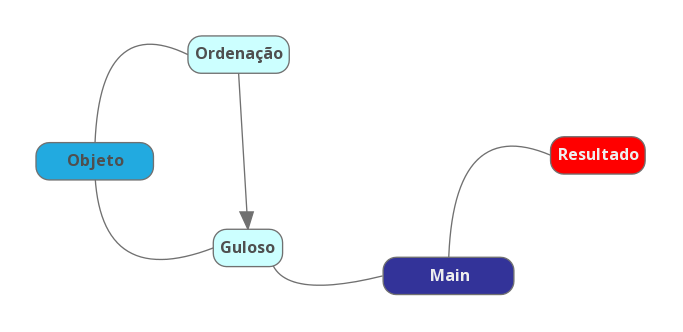
\includegraphics[keepaspectratio=true,scale=0.8]
    	{img/GULOSO.png}
    \label{fig:elementos}
\end{figure}


%O nome do capítulo, apêndice e anexo deve ser sempre em maíuscula e, das seções, em com a letra de cada palavra em maiúscula (exceto preposições e artigos).

\section{Algoritmo de Tentativa e Erro}
\label{sec:textual}







\subsection{Exemplo de Seção de Nível 2}
\subsubsection{Exemplo de Seção de Nível 3}
\subsubsubsection{Exemplo de Seção de Nível 4}

Segundo a \cite{abntTxtAcad2011}, a numeração dos elementos textuais, quando utilizado apenas a frente da folha, deverá ser apresentada no canto direito superior. Quando, no TCC, utiliza-se a frente e o verso da folha, a frente deverá possuir a numeração no canto direito superior e, o verso, no canto esquerdo superior.

\begin{figure}[htb!]
    \centering
    \caption{Desenho feito por Daniel Hasan Dalip.}
    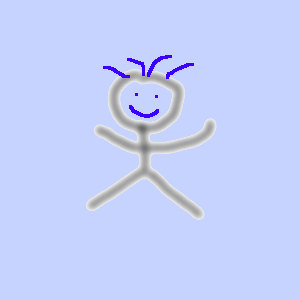
\includegraphics[keepaspectratio=true,scale=0.62]
    	{img/desenho.png}
    \fonte{Daniel Hasan Dalip.}
    \label{fig:desenhoAutor}
\end{figure}

Seguindo as normas  \cite{ibge1993,abntTxtAcad2011}, conforme apresentado nas Figuras~\ref{fig:elementos} e \ref{fig:desenhoAutor}, cada ilustração deve possuir o seu título na parte superior e a fonte de onde foi retirada esta figura na parte inferior. É importante notar que é obrigatório colocar a fonte consultada, mesmo que esta seja o próprio autor. As tabelas devem ser apresentadas conforme a Tabela~\ref{tab:exemploTabela}. Caso queira mais exemplos de tabelas, 
conferir o padrão~\citeonline{ibge1993}. 

\begin{table}[]
\centering
\caption{Exemplo de tabela}
\label{tab:exemploTabela}
\begin{tabular}{lll}
\toprule
Coluna 1                                              & Coluna 2            & Coluna 3 \\ \midrule
21		                                              & 21            		& 212 \\ 
11		                                              & 23            		& 32 \\ 
10		                                              & 11		            & 32 \\ \bottomrule
\end{tabular}
\fonte{Produzido por Daniel H. Dalip e Glívia Angélica.}
\end{table}

As equações podem ser feitas ao longo do texto, por exemplo: $area = \frac{base \times altura}{2}$ ou apresentadas no ambiente \textit{equation}, como na Equação~\ref{eq:testeEquacao}.
\begin{equation}
	area = \frac{base \times altura}{2}
    \label{eq:testeEquacao}
\end{equation}

Finalmente, os textos possuem citações bibliográficas. A padronização das citações são apresentadas por~\citeonline{abntCitacoes2002}. A citação deve ser feita da seguinte forma: caso o nome do autor faça parte do texto, deve-se colocar entre parênteses apenas o ano por exemplo: \citeonline{brin1998anatomy} apresentaram o algoritmo PageRank. Caso contrário, o nome do autor ficará entre parênteses, por exemplo: neste método foi utilizado o algoritmo Page Rank~\cite{brin1998anatomy,abntCitacoes2002}.


\section{Elementos Pós-textuais}
\label{sec:posTextual}

Os elementos pós-textuais são compostos das referências Bibliográficas, Apêndice e Anexos. A ABNT não estabelece um padrão o título dessas seções. No presente documento, seguindo o template do ABNTex2, utilizou-se a fonte \textit{Latin Modern Sans} tamanho 24pt. Deverá haver numeração das páginas. Lembre-se: apêndice são materiais produzidos pelo autor do TCC enquanto anexo são materiais produzidos por outros autores. 
As normas de referencias estão disponíveis em~\cite{abntCitacoes2002}\footnote{Neste site é possível verificar alguns exemplos: \url{http://www.leffa.pro.br/textos/abnt.htm}}.

% ----------------------------------------------------------








% ----------------------------------------------------------
% Finaliza a parte no bookmark do PDF
% para que se inicie o bookmark na raiz
% e adiciona espaço de parte no Sumário
% ----------------------------------------------------------
\phantompart







% ----------------------------------------------------------
% ELEMENTOS PÓS-TEXTUAIS
% ----------------------------------------------------------

%% Baseado no arquivo: 
%% abtex2-modelo-trabalho-academico.tex, v-1.9.6 laurocesar
%% by abnTeX2 group at http://www.abntex.net.br/ 
%% Adaptado para um modelo de TCC (Graduação)

\postextual
% ----------------------------------------------------------

% ----------------------------------------------------------
% Referências bibliográficas
% ----------------------------------------------------------
\bibliography{cefet_mg_decom_abntex2}

% ----------------------------------------------------------
% Glossário
% ----------------------------------------------------------
%
% Consulte o manual da classe abntex2 para orientações sobre o glossário.
%
%\glossary

% ----------------------------------------------------------
% Apêndices
% ----------------------------------------------------------

% ---
% Inicia os apêndices
% ---
\begin{apendicesenv}

% Imprime uma página indicando o início dos apêndices
\partapendices

% ----------------------------------------------------------
\chapter{Título do primeiro apêndice}
% ----------------------------------------------------------

Suspendisse sollicitudin risus et accumsan tempor. Orci varius natoque penatibus et magnis dis parturient montes, nascetur ridiculus mus. Mauris tempor malesuada ligula sed vehicula. Fusce porta magna a blandit aliquet. Nullam auctor tellus et augue lobortis suscipit. Nunc aliquet interdum nisl, at accumsan ante. Donec convallis arcu massa, eu malesuada ex tincidunt quis. Suspendisse turpis orci, auctor et egestas sit amet, ultrices a nisl. Ut interdum metus eu erat facilisis cursus. Maecenas sed dignissim odio, non tempor ipsum. Quisque luctus mi non molestie volutpat.

Class aptent taciti sociosqu ad litora torquent per conubia nostra, per inceptos himenaeos. Proin sed nulla auctor, tempor mauris nec, placerat justo. Vestibulum finibus aliquet ultricies. Nulla facilisi. Ut ante orci, interdum ac sodales vel, porttitor eu justo. Proin laoreet lacinia sapien, non suscipit libero bibendum sit amet. 

% ----------------------------------------------------------
\chapter{Outro Apêndice}
% ----------------------------------------------------------
Nulla facilisi. Ut ante orci, interdum ac sodales vel, porttitor eu justo. Proin laoreet lacinia sapien, non suscipit libero bibendum sit amet. Aliquam orci risus, venenatis et nibh eget, dictum imperdiet ligula. Suspendisse sollicitudin risus et accumsan tempor. Orci varius natoque penatibus et magnis dis parturient montes, nascetur ridiculus mus. Mauris tempor malesuada ligula sed vehicula. Fusce porta magna a blandit aliquet. Nullam auctor tellus et augue lobortis suscipit. Nunc aliquet interdum nisl, at accumsan ante. Donec convallis arcu massa, eu malesuada ex tincidunt quis. Suspendisse turpis orci, auctor et egestas sit amet, ultrices a nisl. Ut interdum metus eu erat facilisis cursus. Maecenas sed dignissim odio, non tempor ipsum. Quisque luctus mi non molestie volutpat.

Nulla facilisi. Ut ante orci, interdum ac sodales vel, porttitor eu justo. Proin laoreet lacinia sapien, non suscipit libero bibendum sit amet.Mauris dictum ante urna, at posuere nulla fermentum id. Proin fermentum odio at elit tristique faucibus. Praesent sit amet facilisis enim, id pulvinar quam. Sed dignissim sem quis tortor tincidunt, mattis blandit eros viverra. Class aptent taciti sociosqu ad litora torquent per conubia nostra, per inceptos himenaeos. Proin sed nulla auctor, tempor mauris nec, placerat justo. Vestibulum finibus aliquet ultricies.  

\end{apendicesenv}
% ---


% ----------------------------------------------------------
% Anexos
% ----------------------------------------------------------

% ---
% Inicia os anexos
% ---
\begin{anexosenv}

% Imprime uma página indicando o início dos anexos
\partanexos

% ---
\chapter{Este é o título do primeiro anexo}
% ---
 Lorem ipsum dolor sit amet, consectetur adipiscing elit. Cras a ultrices dolor. Pellentesque id ex neque. Aliquam orci risus, venenatis et nibh eget, dictum imperdiet ligula. Suspendisse sollicitudin risus et accumsan tempor. Orci varius natoque penatibus et magnis dis parturient montes, nascetur ridiculus mus. Mauris tempor malesuada ligula sed vehicula. Fusce porta magna a blandit aliquet. Nullam auctor tellus et augue lobortis suscipit. Nunc aliquet interdum nisl, at accumsan ante. Donec convallis arcu massa, eu malesuada ex tincidunt quis. Suspendisse turpis orci, auctor et egestas sit amet, ultrices a nisl. Ut interdum metus eu erat facilisis cursus. Maecenas sed dignissim odio, non tempor ipsum. Quisque luctus mi non molestie volutpat.

Mauris dictum ante urna, at posuere nulla fermentum id. Proin fermentum odio at elit tristique faucibus. Praesent sit amet facilisis enim, id pulvinar quam. Sed dignissim sem quis tortor tincidunt, mattis blandit eros viverra. Class aptent taciti sociosqu ad litora torquent per conubia nostra, per inceptos himenaeos. Proin sed nulla auctor, tempor mauris nec, placerat justo. Vestibulum finibus aliquet ultricies. Nulla facilisi. Ut ante orci, interdum ac sodales vel, porttitor eu justo. Proin laoreet lacinia sapien, non suscipit libero bibendum sit amet. 

% ---
\chapter{SEgundo título do segundo anexo}
% ---
Aliquam orci risus, venenatis et nibh eget, dictum imperdiet ligula. Suspendisse sollicitudin risus et accumsan tempor. Orci varius natoque penatibus et magnis dis parturient montes, nascetur ridiculus mus. Mauris tempor malesuada ligula sed vehicula. Fusce porta magna a blandit aliquet. Nullam auctor tellus et augue lobortis suscipit. Nunc aliquet interdum nisl, at accumsan ante. Donec convallis arcu massa, eu malesuada ex tincidunt quis. Suspendisse turpis orci, auctor et egestas sit amet, ultrices a nisl. Ut interdum metus eu erat facilisis cursus. Maecenas sed dignissim odio, non tempor ipsum. Quisque luctus mi non molestie volutpat.

Praesent sit amet facilisis enim, id pulvinar quam. Sed dignissim sem quis tortor tincidunt, mattis blandit eros viverra. Class aptent taciti sociosqu ad litora torquent per conubia nostra, per inceptos himenaeos. Proin sed nulla auctor, tempor mauris nec, placerat justo. Vestibulum finibus aliquet ultricies. Nulla facilisi. Ut ante orci, interdum ac sodales vel, porttitor eu justo. Proin laoreet lacinia sapien, non suscipit libero bibendum sit amet. 



\end{anexosenv}



\end{document}
